\hspace*{12pt}Los resultados obtenidos para el diagrama HR en la vecindad solar es el que sigue:
	
	\begin{figure}[!htbp]
		\centering
		\title{\textbf{HR Diagram\vspace{2ex}}}
		\begin{center}
			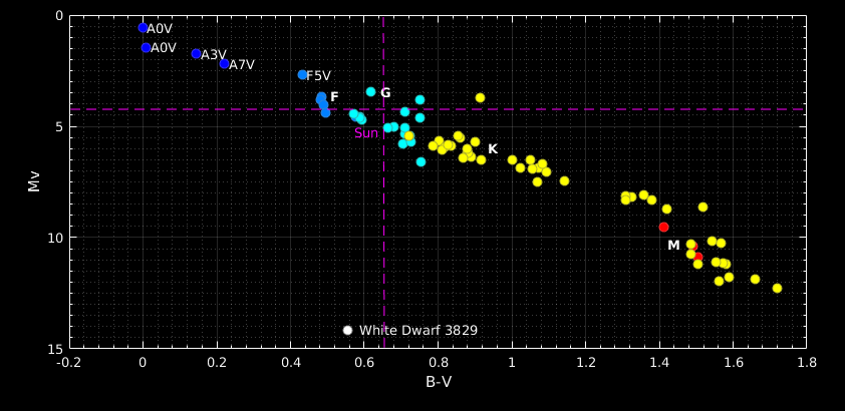
\includegraphics[width=15cm]{Figures/HRdiagram2.png}
		\end{center}
		\caption{\footnotesize{En el siguiente diagrama se han representado ambas cantidades en "magnitudes". Se ha diferenciado el tipo espectral de cada estrella mediante el color del punto que la representa y se ha marcado como referencia la posici\'{o}n del Sol en el diagrama.}}
		\label{HRdiag}
		\end{figure}
		
	Para hacer un an\'{a}lisis de los resultados obtenidos conviene fijarse en los cuadrantes delimitados por las l\'{i}neas solares (Sun en la Figura \ref{HRdiag}). Lo primero que destaca en esta separaci\'{o}n es la diferencia que hay en el n\'{u}mero de estrellas en los cuadrantes superior izquierdo e inferior derecho. Esto puede explicarse facilmente si se tiene en cuenta la vida media asociada a las estrellas de tipo A y F frente a la vida media de las estrellas de tipo K. En general, las estrellas de tipo A y F tienen una vida media mucho menor que las de tipo K, lo que explica c\'{o}mo una distribuci\'{o}n que podemos postular aleatoria de estrellas inicial acaba por consistir en un gran n\'{u}mero de estrellas K y un menor n\'{u}mero del resto seg\'{u}n las de tipo A y F van consumiendose.
	\\ \hspace*{12pt}  Por otro lado, el Sol es una estrellade tipo G, como podemos ver en el diagrama. Esto explica la distribuci\'{o}n de luminosidades obtenida en la Figura \ref{Lhist} donde la gran mayor\'{i}a de estrellas se situaban en una luminosidad menor a la del Sol, lo que equivale a estar en los cuadrantes inferiores del Diagrama HR. Las pocas estrellas situadas por encima se corresponden entonces con las estrellas de tipo A, F y las de tipo G que son ligeramente más luminosas que el Sol. 
